% Baccalauréat malgache, série C, 2011 : corrigé.
\TCDBacAttribution{C}{2011}
\providecommand{\cm}{~\mathrm{cm}}
\providecommand{\Plan}{(\mathscr{P})}
\providecommand{\dx}{~\mathrm{d}x}
\providecommand{\dt}{\mathrm{d}t}
\providecommand{\Ouv}{(O;\vec{u},\vec{v})}
\providecommand{\mes}[2]{\mathrm{mes}\left( \widehat{ \overrightarrow{#1} ; \overrightarrow{#2} } \right)}
\providecommand{\D}{(\mathscr{D})}
\providecommand{\Courbe}{(\mathscr{C})}
\providecommand{\Courben}{(\mathscr{C}_n)}
\providecommand{\CourbeU}{(\mathscr{C}_1)}
\providecommand{\CourbeD}{(\mathscr{C}_2)}
\providecommand{\bary}[1]{\mathrm{bar}\left\lbrace #1 \right\rbrace}
\providecommand{\congru}[3]{#1 \equiv #2 \quad \left[ \mathrm{mod}~#3\right]}
\providecommand{\Angl}[2]{\left( \widehat{ \overrightarrow{#1} , \overrightarrow{#2} } \right)}
%
%%%%%%%%%%%%%%%%%%%%%%%%%%%%%%%%%%%%%%%%%%%%%%%%%%%%%%%%%%%%%%%%%%%%%%%%%%%%%%%%%%%%%%%%%%%%%%%%%%%%%%%%%%%%%%%%%%%%%%%%%%%%%%%%
\noindent \underline{\textsc{\textbf{Exercice}}} (4 points)
\begin{description}
	\item[A- Probabilité.]
	\begin{enumerate}
		\item \vln{Probabilités élémentaires :}
			Le dé est parfait : chaque face a la probabilité $\frac{1}{6}$. Une face porte $0$, deux portent $1$, trois portent $2$.
			\par\noindent\ansbox{$P_0 = \frac{1}{6}$, $P_1 = \frac{1}{3}$, $P_2 = \frac{1}{2}$.}
		\item Les trois lancers sont indépendants : la probabilité d'une suite de résultats est le produit des probabilités.
		\begin{description}
			\item[$A$ :] \vln{Somme égale à $4$ :}
				Avec des numéros $0$, $1$, $2$, on a $4 = 2 + 2 + 0 = 2 + 1 + 1$ (à l'ordre près).
				Les suites formées de $\{2,2,0\}$ sont au nombre de $3$ (place du $0$), de même pour $\{2,1,1\}$ (place du $2$).
				$P(A) = 3 \times \left(\frac{1}{2}\right)^2 \times \frac{1}{6} + 3 \times \frac{1}{2} \times \left(\frac{1}{3}\right)^2 = \frac{1}{8} + \frac{1}{6}$,
				soit \par\noindent\ansbox{$P(A) = \frac{7}{24}$.}
			\item[$B$ :] \vln{Exactement deux fois le numéro $1$ :}
				Loi binomiale de paramètres $3$ et $\frac{1}{3}$ : $P(B) = \Comb{3}{2}\left(\frac{1}{3}\right)^2 \cdot \frac{2}{3} = \frac{6}{27}$,
				soit \par\noindent\ansbox{$P(B) = \frac{2}{9}$.}
			\item[$C$ :] \vln{Trois numéros différents :}
				Les trois numéros $0$, $1$, $2$ apparaissent chacun une fois, dans l'un des $3! = 6$ ordres :
				$P(C) = 6 \times \frac{1}{6} \times \frac{1}{3} \times \frac{1}{2}$, soit \par\noindent\ansbox{$P(C) = \frac{1}{6}$.}
		\end{description}
	\end{enumerate}
	\item[B- Arithmétique.]
	\begin{enumerate}
		\item
		\begin{enumerate}
			\item \vln{Conversion en base dix :}
				$a = 1 \cdot 2^6 + 0 \cdot 2^5 + 1 \cdot 2^4 + 1 \cdot 2^3 + 1 \cdot 2^2 + 0 \cdot 2 + 1 = 64 + 16 + 8 + 4 + 1$ : \par\noindent\ansbox{$a = 93$.}
			\item \vln{Conversion en binaire :}
				$54 = 2 \times 27 + 0$, $27 = 2 \times 13 + 1$, $13 = 2 \times 6 + 1$, $6 = 2 \times 3 + 0$, $3 = 2 \times 1 + 1$, $1 = 2 \times 0 + 1$.
				On lit les restes de bas en haut : \par\noindent\ansbox{$b = \overline{(110110)_2}$} ($32 + 16 + 4 + 2 = 54$).
		\end{enumerate}
		\item
		\begin{enumerate}
			\item \vln{Tables de $\mathbb{Z}/5\mathbb{Z}$ :}
				\[
				\begin{array}{c|ccccc}
					+ & \bar{0} & \bar{1} & \bar{2} & \bar{3} & \bar{4} \\ \hline
					\bar{0} & \bar{0} & \bar{1} & \bar{2} & \bar{3} & \bar{4} \\
					\bar{1} & \bar{1} & \bar{2} & \bar{3} & \bar{4} & \bar{0} \\
					\bar{2} & \bar{2} & \bar{3} & \bar{4} & \bar{0} & \bar{1} \\
					\bar{3} & \bar{3} & \bar{4} & \bar{0} & \bar{1} & \bar{2} \\
					\bar{4} & \bar{4} & \bar{0} & \bar{1} & \bar{2} & \bar{3}
				\end{array}
				\qquad
				\begin{array}{c|ccccc}
					\times & \bar{0} & \bar{1} & \bar{2} & \bar{3} & \bar{4} \\ \hline
					\bar{0} & \bar{0} & \bar{0} & \bar{0} & \bar{0} & \bar{0} \\
					\bar{1} & \bar{0} & \bar{1} & \bar{2} & \bar{3} & \bar{4} \\
					\bar{2} & \bar{0} & \bar{2} & \bar{4} & \bar{1} & \bar{3} \\
					\bar{3} & \bar{0} & \bar{3} & \bar{1} & \bar{4} & \bar{2} \\
					\bar{4} & \bar{0} & \bar{4} & \bar{3} & \bar{2} & \bar{1}
				\end{array}
				\]
			\item \vln{Résolution du système :}
				On multiplie la première équation par $\bar{2}$ : $\bar{6}x + \bar{4}y = \bar{2}$, soit $x + \bar{4}y = \bar{2}$.
				En la retranchant de la seconde : $(\bar{2}x + \bar{4}y) - (x + \bar{4}y) = \bar{3} - \bar{2}$, d'où $x = \bar{1}$.
				Alors $\bar{3} + \bar{2}y = \bar{1}$, $\bar{2}y = -\bar{2} = \bar{3}$ et, en multipliant par $\bar{3}$ (inverse de $\bar{2}$), $y = \bar{9} = \bar{4}$.
				Vérification : $\bar{3} + \bar{8} = \bar{11} = \bar{1}$ et $\bar{2} + \bar{16} = \bar{18} = \bar{3}$.
				\par\noindent\ansbox{$S = \{(\bar{1} \, ; \bar{4})\}$.}
			\item \vln{Équation $x^2 - x - \bar{2} = \bar{0}$ :}
				$(x - \bar{2})(x + \bar{1}) = x^2 - x - \bar{2}$. Comme $5$ est premier, un produit est nul dans $\mathbb{Z}/5\mathbb{Z}$ si et seulement si l'un des facteurs est nul
				(la table de multiplication n'a pas de $\bar{0}$ hors de la ligne et de la colonne de $\bar{0}$).
				Donc $x = \bar{2}$ ou $x = -\bar{1} = \bar{4}$. \par\noindent\ansbox{$S = \{\bar{2} \, ; \bar{4}\}$.}
		\end{enumerate}
	\end{enumerate}
\end{description}
%%%%%%%%%%%%%%%%%%%%%%%%%%%%%%%%%%%%%%%%%%%%%%%%%%%%%%%%%%%%%%%%%%%%%%%%%%%%%%%%%%%%%%%%%%%%%%%%%%%%%%%%%%%%%%%%%%%%%%%%%%%%%%%%
\noindent \underline{\textsc{\textbf{PROBLEME I}}} (7 points) \newline
Le triangle $ABC$ est équilatéral direct de côté $4\cm$ ; $E$ est le symétrique de $A$ par rapport au milieu $O$ de $[BC]$.
\begin{description}
	\item[Partie A]
	\begin{enumerate}
		\item \vln{Figure en vraie grandeur} (les points $G$, $I$, $I'$ et la droite $\D$ sont construits plus loin) :
			\begin{center}
			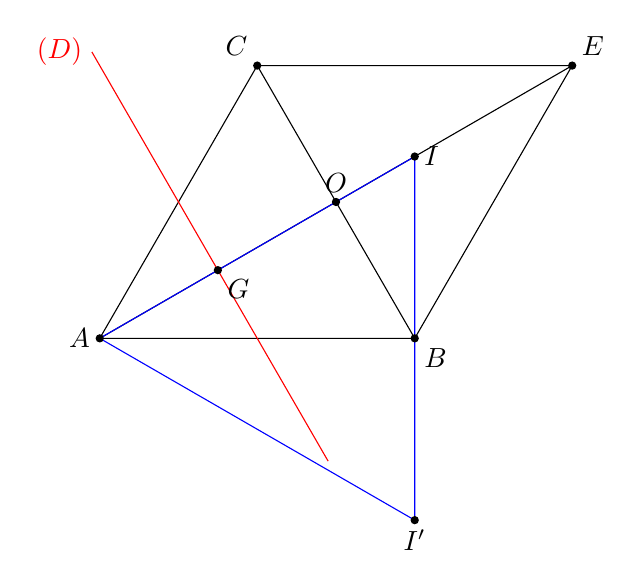
\begin{tikzpicture}[x=1cm,y=1cm]
				\coordinate (A) at (0,0); \coordinate (B) at (4,0); \coordinate (C) at (2,3.464); \coordinate (E) at (6,3.464);
				\coordinate (O) at (3,1.732); \coordinate (G) at (1.5,0.866); \coordinate (I) at (4,2.309); \coordinate (I') at (4,-2.309);
				\draw (A) -- (B) -- (E) -- (C) -- cycle; \draw (A) -- (E); \draw (B) -- (C);
				\draw[blue] (A) -- (I) -- (I') -- cycle;
				\draw[red] (2.9,-1.559) -- (-0.1,3.637) node[left] {$\D$};
				\foreach \P/\pos in {A/left,B/below right,C/above left,E/above right,O/above,G/below right,I/right,I'/below}
					\fill (\P) circle (1.5pt) node[\pos] {$\P$};
			\end{tikzpicture}
			\end{center}
		\item
		\begin{enumerate}
			\item \vln{Barycentre $G$ :}
				La somme des poids $2 + 1 + 1 = 4$ est non nulle : $G$ existe.
				$O$ est le milieu de $[BC]$, donc $O = \bary{(B,1);(C,1)}$ et, par associativité, $G = \bary{(A,2);(O,2)}$.
				\par\noindent\ansbox{$G$ est le milieu de $[OA]$.}
			\item \vln{Vecteur constant :}
				$-2\overrightarrow{MA} + \overrightarrow{MB} + \overrightarrow{MC} = -2\overrightarrow{MA} + \left(\overrightarrow{MA} + \overrightarrow{AB}\right) + \left(\overrightarrow{MA} + \overrightarrow{AC}\right) = \overrightarrow{AB} + \overrightarrow{AC}$.
				\par\noindent\ansbox{$-2\overrightarrow{MA} + \overrightarrow{MB} + \overrightarrow{MC} = \overrightarrow{AB} + \overrightarrow{AC} = 2\overrightarrow{AO} = \overrightarrow{AE}$.}
			\item \vln{Ensemble $\D$ :}
				$2\overrightarrow{MA} + \overrightarrow{MB} + \overrightarrow{MC} = 4\overrightarrow{MG}$ ($G$ barycentre). La condition devient
				$4\overrightarrow{MG} \cdot \overrightarrow{AE} = 0$, soit $\overrightarrow{GM} \perp \overrightarrow{AE}$.
				\par\noindent\ansbox{$\D$ est la droite passant par $G$ et perpendiculaire à $(AE)$,}
				c'est-à-dire la parallèle à $(BC)$ passant par $G$ (les diagonales du losange sont perpendiculaires). Elle est représentée sur la figure.
		\end{enumerate}
		\item
		\begin{enumerate}
			\item \vln{Triangle $IAI'$ :}
				$S(I) = I$ et $S(A) = B$ : $IB = \frac{1}{2} IA$ et $\Angl{IA}{IB} = \frac{\pi}{3}$.
				$B$ est le milieu de $[II']$, donc $\overrightarrow{II'} = 2\overrightarrow{IB}$ : $II' = 2IB = IA$ et $\Angl{IA}{II'} = \Angl{IA}{IB} = \frac{\pi}{3}$.
				Le triangle $IAI'$ est isocèle en $I$ avec un angle au sommet de $\frac{\pi}{3}$ : il est équilatéral, et direct car $\Angl{IA}{II'} = +\frac{\pi}{3}$.
				\par\noindent\ansbox{$IAI'$ est un triangle équilatéral direct.}
			\item \vln{$\Angl{AB}{AI} = \frac{\pi}{6}$ :}
				Dans le triangle équilatéral $IAI'$, $B$ est le milieu de $[II']$ : $(AB)$ est la médiane, donc aussi la bissectrice issue de $A$ et la hauteur.
				Ainsi $\widehat{BAI} = \frac{1}{2} \cdot \frac{\pi}{3} = \frac{\pi}{6}$ et $(IB) \perp (AB)$.
				Le triangle $AI'I$ étant direct, $\Angl{AI'}{AI} = \frac{\pi}{3}$ et $(AB)$ bissectrice donne $\Angl{AB}{AI} = \frac{\pi}{6}$.
				\par\noindent\ansbox{$\mes{AB}{AI} = \frac{\pi}{6}$.}
			\item \vln{Construction de $I$ et $I'$ :}
				$I$ est l'intersection de la perpendiculaire à $(AB)$ en $B$ et de la demi-droite d'origine $A$ faisant l'angle $\frac{\pi}{6}$ avec $[AB)$, c'est-à-dire la demi-droite $[AO)$
				(car $\Angl{AB}{AO} = \frac{\pi}{6}$) ; $I'$ est le symétrique de $I$ par rapport à $B$. Voir la figure.
		\end{enumerate}
	\end{enumerate}
	\item[Partie B]
	\begin{enumerate}
		\item
		\begin{enumerate}
			\item \vln{Affixes de $A$ et $B$ :}
				\ansbox{$z_A = 0$ et $z_B = 4$.}
			\item \vln{Affixe de $C$ :}
				$AC = 4$ et $\Angl{u}{AC} = \Angl{AB}{AC} = \frac{\pi}{3}$ : \par\noindent\ansbox{$|z_C| = 4$, $\arg z_C = \frac{\pi}{3}$, $z_C = 2 + 2\sqrt{3}\, i$.}
			\item \vln{Affixe de $O$ :}
				$z_O = \frac{z_B + z_C}{2}$, soit \par\noindent\ansbox{$z_O = 3 + \sqrt{3}\, i$.}
		\end{enumerate}
		\item
		\begin{enumerate}
			\item \vln{Expression complexe de $S$ :}
				$S : z' = kz + b$ avec $k = \frac{1}{2}\expo{i\frac{\pi}{3}} = \frac{1}{4} + \frac{\sqrt{3}}{4} i$ ; $S(A) = B$ donne $b = 4$.
				\par\noindent\ansbox{$S : z' = \left(\frac{1}{4} + \frac{\sqrt{3}}{4} i\right) z + 4$.}
			\item \vln{Centre $I$ :}
				$z_I = k z_I + 4 \iff z_I = \frac{4}{\frac{3}{4} - \frac{\sqrt{3}}{4} i} = \frac{16}{3 - i\sqrt{3}} = \frac{16(3 + i\sqrt{3})}{12}$.
				\par\noindent\ansbox{$z_I = 4 + \frac{4\sqrt{3}}{3}\, i$.}
			\item \vln{Vérifications :}
				$z_I = \frac{4}{3}(3 + i\sqrt{3}) = \frac{4}{3} z_O$, donc \par\noindent\ansbox{$\frac{z_I}{z_O} = \frac{4}{3}$ est réel.}
				$\frac{z_B - z_I}{z_B - z_A} = \frac{-\frac{4\sqrt{3}}{3} i}{4}$, donc \par\noindent\ansbox{$\frac{z_B - z_I}{z_B - z_A} = -\frac{\sqrt{3}}{3}\, i$ est imaginaire pur.}
			\item \vln{Conséquences :}
				$\frac{z_I - z_A}{z_O - z_A} \in \mathbb{R}$ : les vecteurs $\overrightarrow{AI}$ et $\overrightarrow{AO}$ sont colinéaires.
				\par\noindent\ansbox{$I$, $O$, $A$ sont alignés.}
				$\frac{z_B - z_I}{z_B - z_A}$ imaginaire pur non nul : $\overrightarrow{IB} \perp \overrightarrow{AB}$.
				\par\noindent\ansbox{Les droites $(IB)$ et $(AB)$ sont perpendiculaires,}
				ce qui confirme la construction de la partie A.
		\end{enumerate}
	\end{enumerate}
\end{description}
%%%%%%%%%%%%%%%%%%%%%%%%%%%%%%%%%%%%%%%%%%%%%%%%%%%%%%%%%%%%%%%%%%%%%%%%%%%%%%%%%%%%%%%%%%%%%%%%%%%%%%%%%%%%%%%%%%%%%%%%%%%%%%%%
\noindent \underline{\textsc{\textbf{PROBLEME II}}} (9 points)
\begin{description}
	\item[Partie A :]
	\begin{enumerate}
		\item \vln{Limites :}
			En $-\infty$ : $\expo{\frac{x}{2}} \to 0$ et $-x - 1 \to +\infty$, donc \par\noindent\ansbox{$\lim_{x\to-\infty} f(x) = +\infty$.}
			En $+\infty$ : avec $X = \frac{x}{2}$, $f(x) = \expo{X} - 2X - 1 = X\left(\frac{\expo{X}}{X} - 2\right) - 1$ et $\frac{\expo{X}}{X} \to +\infty$,
			donc \par\noindent\ansbox{$\lim_{x\to+\infty} f(x) = +\infty$.}
		\item
		\begin{enumerate}
			\item \vln{Variations :}
				$f'(x) = \frac{1}{2}\expo{\frac{x}{2}} - 1$ ; $f'(x) > 0 \iff \expo{\frac{x}{2}} > 2 \iff x > 2\ln 2$.
				$f(2\ln 2) = 2 - 2\ln 2 - 1 = 1 - 2\ln 2 \approx -0{,}39$.
				\[
				\begin{array}{c|ccccc}
					x & -\infty & & 2\ln 2 & & +\infty \\ \hline
					f'(x) & & - & 0 & + & \\ \hline
					 & +\infty & & & & +\infty \\
					f & & \searrow & & \nearrow & \\
					 & & & 1 - 2\ln 2 & &
				\end{array}
				\]
			\item \vln{Asymptote $\D$ :}
				$f(x) - (-x - 1) = \expo{\frac{x}{2}} \to 0$ quand $x \to -\infty$.
				\par\noindent\ansbox{$\D : y = -x - 1$ est asymptote à $\Courbe$ en $-\infty$ ;}
				de plus $\Courbe$ est au-dessus de $\D$ car $\expo{\frac{x}{2}} > 0$.
			\item \vln{Solutions de $f(x) = 0$ :}
				$f(0) = 1 - 0 - 1 = 0$. Sur $]-\infty ; 2\ln 2]$, $f$ est strictement décroissante, donc $0$ y est la seule solution ($0 < 2\ln 2$).
				Sur $[2\ln 2 ; +\infty[$, $f$ est continue et strictement croissante de $1 - 2\ln 2 < 0$ vers $+\infty$ : une unique solution $\alpha$.
				$f(2) = e - 3 \approx -0{,}28 < 0$ et $f(3) = \expo{\frac{3}{2}} - 4 \approx 0{,}48 > 0$.
				\par\noindent\ansbox{$f(x) = 0$ a exactement deux solutions, $0$ et $\alpha$, avec $2 < \alpha < 3$ ($\alpha \approx 2{,}51$).}
		\end{enumerate}
		\item \vln{Tracé (unité $2\cm$ réduite à $1{,}2\cm$ sur la figure) :}
			Valeurs : $f(-4) \approx 3{,}14$ ; $f(-2) \approx 1{,}37$ ; $f(-1) \approx 0{,}61$ ; $f(1) \approx -0{,}35$ ; $f(3{,}5) \approx 1{,}26$.
			\begin{center}
			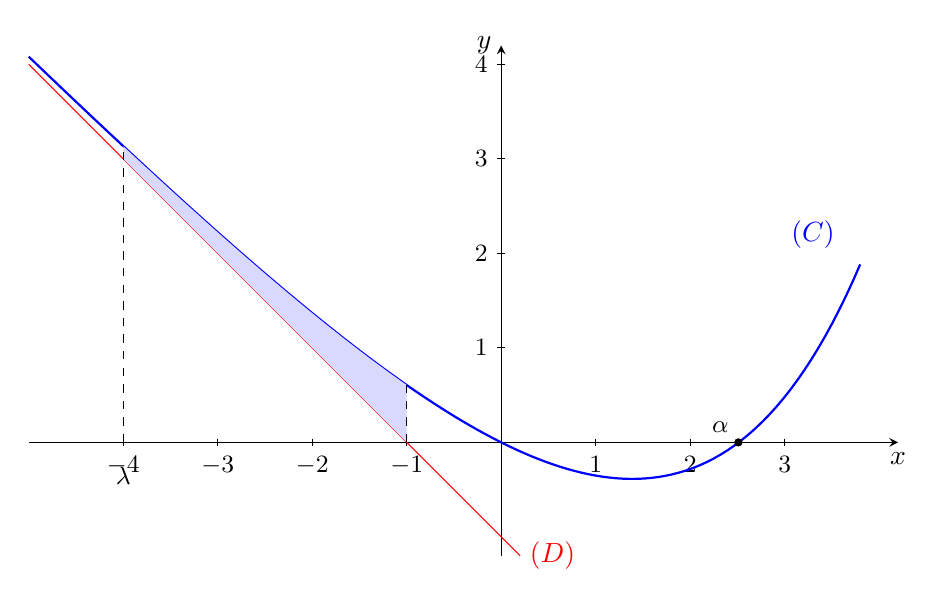
\begin{tikzpicture}[x=1.2cm,y=1.2cm,>=stealth]
				\draw[->] (-5,0) -- (4.2,0) node[below] {$x$};
				\draw[->] (0,-1.2) -- (0,4.2) node[left] {$y$};
				\foreach \t in {-4,-3,-2,-1,1,2,3} \draw (\t,0.04) -- (\t,-0.04) node[below] {\small $\t$};
				\foreach \t in {1,2,3,4} \draw (0.04,\t) -- (-0.04,\t) node[left] {\small $\t$};
				\draw[red] (-5,4) -- (0.2,-1.2) node[right] {$\D$};
				\draw[blue,thick] plot[domain=-5:3.8,samples=120] (\x,{exp(\x/2)-\x-1});
				\fill[blue!15] (-4,3) -- plot[domain=-4:-1,samples=30] (\x,{exp(\x/2)-\x-1}) -- (-1,0) -- cycle;
				\draw[dashed] (-4,0) -- (-4,3.135) (-1,0) -- (-1,0.607);
				\node at (-4,-0.35) {\small $\lambda$};
				\node[blue] at (3.3,2.2) {$\Courbe$};
				\fill (2.51,0) circle (1.5pt) node[above left] {\small $\alpha$};
			\end{tikzpicture}
			\end{center}
		\item
		\begin{enumerate}
			\item \vln{Aire $A(\lambda)$ :}
				Sur $[\lambda ; -1]$, $\Courbe$ est au-dessus de $\D$ et $f(x) - (-x-1) = \expo{\frac{x}{2}}$.
				L'unité d'aire vaut $2 \times 2 = 4\,\mathrm{cm}^2$ :
				$A(\lambda) = 4\int_\lambda^{-1} \expo{\frac{x}{2}}\dx = 4\left[2\expo{\frac{x}{2}}\right]_\lambda^{-1}$.
				\par\noindent\ansbox{$A(\lambda) = 8\left(\expo{-\frac{1}{2}} - \expo{\frac{\lambda}{2}}\right)\ \mathrm{cm}^2$.}
			\item \vln{Limite :}
				$\expo{\frac{\lambda}{2}} \to 0$ quand $\lambda \to -\infty$ :
				\par\noindent\ansbox{$\lim_{\lambda\to-\infty} A(\lambda) = 8\expo{-\frac{1}{2}} = \frac{8}{\sqrt{e}} \approx 4{,}85\ \mathrm{cm}^2$.}
		\end{enumerate}
	\end{enumerate}
	\item[Partie B :]
	\begin{enumerate}
		\item \vln{Variations de $g$ :}
			$g'(x) = \frac{2}{x+1} > 0$ sur $]-1;+\infty[$ ; $\lim_{x\to -1^+} g(x) = -\infty$, $\lim_{x\to+\infty} g(x) = +\infty$.
			\par\noindent\ansbox{$g$ est strictement croissante sur $]-1;+\infty[$.}
		\item \vln{$g(\alpha) = \alpha$ :}
			$f(\alpha) = 0 \iff \expo{\frac{\alpha}{2}} = \alpha + 1$ ; comme $\alpha + 1 > 0$, on prend le logarithme : $\frac{\alpha}{2} = \ln(\alpha + 1)$, soit $\alpha = 2\ln(\alpha+1)$.
			\par\noindent\ansbox{$g(\alpha) = \alpha$.}
		\item \vln{$g([2;+\infty[) \subset ]2;+\infty[$ :}
			$g$ est croissante, donc pour $x \geq 2$ : $g(x) \geq g(2) = 2\ln 3 \approx 2{,}20 > 2$ (car $\ln 3 > 1$).
			\par\noindent\ansbox{Pour $x \geq 2$, $g(x) > 2$.}
		\item
		\begin{enumerate}
			\item \vln{Majoration de $|g'|$ :}
				Pour $x \geq 2$, $x + 1 \geq 3$, donc $0 < g'(x) = \frac{2}{x+1} \leq \frac{2}{3}$.
				\par\noindent\ansbox{$|g'(x)| \leq \frac{2}{3}$ pour tout $x \geq 2$.}
			\item \vln{Inégalités :}
				$U_n$ et $\alpha$ sont dans $[2;+\infty[$, où $|g'| \leq \frac{2}{3}$ ; l'inégalité des accroissements finis donne
				$|g(U_n) - g(\alpha)| \leq \frac{2}{3}|U_n - \alpha|$, soit
				\par\noindent\ansbox{$|U_{n+1} - \alpha| \leq \frac{2}{3}|U_n - \alpha|$.}
				Par récurrence $|U_n - \alpha| \leq \left(\frac{2}{3}\right)^n|U_0 - \alpha|$ et $|U_0 - \alpha| = 3 - \alpha < 1$ :
				\par\noindent\ansbox{$|U_n - \alpha| \leq \left(\frac{2}{3}\right)^n$.}
			\item \vln{Convergence :}
				$\left(\frac{2}{3}\right)^n \to 0$, donc \par\noindent\ansbox{$(U_n)$ converge vers $\ell = \alpha$.}
			\item \vln{Entier $p$ :}
				Il suffit que $\left(\frac{2}{3}\right)^n \leq 10^{-4}$, soit $n \geq \frac{4\ln 10}{\ln\frac{3}{2}} \approx 22{,}7$.
				\par\noindent\ansbox{$p = 23$ : pour $n \geq 23$, $|U_n - \alpha| \leq 10^{-4}$.}
		\end{enumerate}
	\end{enumerate}
\end{description}
